\documentclass{ltjsarticle}
\usepackage{amsmath,amssymb}
\usepackage{bm}
\usepackage{here}
\usepackage{graphicx}
\usepackage{hyperref}
\usepackage{physics}
\usepackage{subcaption}
\usepackage{tikz}
\usepackage{xcolor}
\usepackage{algorithm,algpseudocode}
\usepackage[sorting=none]{biblatex}
\addbibresource{references.bib}

\usetikzlibrary{intersections, calc, arrows}

\definecolor{cud_red}{RGB}{255,75,0}
\definecolor{cud_green}{RGB}{3,175,122}
\definecolor{cud_blue}{RGB}{0,90,255}
\definecolor{cud_sky}{RGB}{77,196,255}
\hypersetup{
    colorlinks=true,
    linkcolor=cud_blue,
    citecolor=cud_blue,
    filecolor=cud_red,      
    urlcolor=cud_green,
}

\algnewcommand{\Break}{\textbf{break}}
\renewcommand{\algorithmicrequire}{\textbf{Input:}}
\renewcommand{\algorithmicensure}{\textbf{Output:}}

\begin{document}
\title{Julia言語でFEMを書いてポテンシャル流れを解く}
\author{きゅーしす}
\maketitle
\begin{abstract}
    Julia言語は近年開発された言語で, 簡潔に表現されたコードで高速に実行できる特徴をもつ. 
    これらの特徴からデータサイエンスや機械学習, 科学技術計算での利用が広がっている. 
    この例として, 筆者が自作した2次元Poisson方程式の有限要素法(Finite Element method, FEM)のコードを取り上げ, 
    Julia言語の特徴を実例を交えながら示す. 
\end{abstract}


\section{イントロダクション}
Julia言語は近年開発された言語で, 自由なライセンスで高速で簡潔に記述でき, 
強力なマクロがあり, 汎用性を持ち, 統計や科学技術計算にも強い\cite{Bezanson2012}. 
また, パッケージ管理も十分に整備されており, 
Pythonをはじめとしたユーザーの多い言語には及ばないものの, パッケージは充実している. 

汎用性がありつつも科学技術計算に強いという特徴や
パッケージ管理システムが整備されていることは数値解析に大いに役立つ.
たとえば, 線形代数や複素数が簡潔な記法で記述でき, 
従来の数値計算で使われているC/C++やFortranの泣き所であったファイルの入出力や結果のプロットまで一貫してJulia言語のみで構築できる.
一方で, C/C++やFortranはパッケージ管理システムに乏しく, 
その上メンテナンス性が高いとはとても言えない\footnote{個人の見解です. 異論は認めます}. 
さらに, プロファイリングや並列計算も便利な記法があり, 高性能計算(HPC)での利用も広がっている.

Julia言語は利点も多数あるが, 新しいプログラミング言語であるので情報が少ない. 
海外では利用例が増えているが, 日本での利用例が少ないのも課題である. 
科学技術計算での利用はは尚更その傾向が強い. 
この記事で日本語のJulia言語での科学技術計算の情報を少しでも提供できたら幸いである. 

続いて構成を示す. 
はじめに, 今回解くポテンシャル流れについて概説する. 
次に有限要素法での近似と離散化, アルゴリズムについて概説する. 
その後にJulia言語の特徴と書いたプログラムの実装を示す. 
そして計算結果と考察をし, 記事全体のまとめを記す. 

\section{ポテンシャル流れとは}
今回解く問題はポテンシャル流れと呼ばれる. 
ポテンシャル流れの「ポテンシャル」とは何者なのか, 
支配方程式は何なのか,
文献\cite{Kanbe1995}を参考にその導出を行って概説する. 

ポテンシャル流れの対象となるのは非圧縮完全流体と呼ばれるものである. 
性質を以下に列挙する. 
\begin{itemize}
    \item \textbf{非圧縮}とは流体の密度が変わらないこと($\pdv*{\rho}{t}=0$)\footnote{非圧縮な流体は音速が無限大になるので現実世界には存在しない}
    \item \textbf{完全流体}は非粘性である(粘性がない)
    \item 完全流体は非熱伝導性である(熱を一切伝えない)
\end{itemize}
なお, 完全流体の定義は神部ら\cite{Kanbe1995}の定義を採用した. 
非圧縮完全流体の支配方程式は以下に示す連続の式(式\eqref{eq:continuity})とEulerの運動方程式(式\eqref{eq:euler})である. 
\begin{align}
    \nabla\cdot\bm{u} &= 0 \label{eq:continuity} \\
    \pdv{\bm{u}}{t} +(\bm{u}\cdot\nabla)\bm{u} &= -\frac{1}{\rho}\nabla p + \bm{f} \label{eq:euler}
\end{align}
ここで速度を$\bm{u}$, 密度を$\rho$, 圧力を$p$, 外力を$\bm{f}$とした.
Euler方程式は非圧縮かつ完全流体という仮定を入れたにもかかわらず, 解析的な解を求めることはほぼ不可能である
\footnote{この問題は大変難しく, 未だ解析解があるかどうかすらわかっていない}.
さらに幾つかの仮定を導入してより簡単な方程式を導出し, 流れを近似的に求めることを行いたい.

まず, 流れ場が時間に対して変化しない定常状態($\pdv*{\bm{u}}{t}=0$)を仮定する.
このとき, Euler方程式は以下のようになる.
\begin{align}
    (\bm{u}\cdot\nabla)\bm{u} &= -\frac{1}{\rho}\nabla p + \bm{f} \label{eq:euler:steady}
\end{align}
次に, 渦度$\bm{\omega}$を速度の回転$\nabla\cdot\bm{u}$と定義する.
このとき, 外力がポテンシャル$\chi$によるもので$\bm{f}=-\nabla \chi$と表されれば,
式\eqref{eq:euler:steady}は以下のように変形できる.
\begin{align}
    \bm{\omega}\times\bm{u}=-\nabla\qty(\frac{1}{2}|\bm{u}|^2 + \frac{p}{\rho}+\chi)
    \label{eq:euler:steady:vorticity}
\end{align}
この式の右辺は速度と渦度のそれぞれに直交したベクトルである.
つまり, 式の値は流線($\bm{u}$にそった線)と渦線($\bm{\omega}$にそった線)それぞれの上で
$\frac{1}{2}|\bm{u}|^2 + \frac{p}{\rho}+\chi$が変化しないことを示している.
よって, 渦線もしくは流線に沿って
\begin{align}
    \frac{1}{2}|\bm{u}|^2 + \frac{p}{\rho}+\chi=\mathrm{constant}, \quad\mathrm{渦線もしくは流線に沿って}
    \label{eq:bernoulli}
\end{align}
が成り立つ. これをBernoulliの定理という.
詳細は神部ら\cite{Kanbe1995}を参照されたい. 

次に\textbf{渦なし}という概念を導入する. 渦なしとはいたるところで
渦度が0であることを意味する. 
渦なしの場合, Stokesの定理より
\begin{align}
    \oint_{C} \bm{u}\cdot\mathrm{d}\bm{l} 
    = \iint_S\nabla\times\bm{u}\cdot\bm{n}\mathrm{d}S =0
    \label{eq:stokes:zero}
\end{align}
が成立する, 
ここで$C$は単純閉曲線で, $S$は$C$を境界とする面である. 
この結果から, 積分路に依存せず, 開始と終点のみで値が決まる.
速度ポテンシャルが存在する\footnote{詳細は付録\ref{appendix:potential}を参照}.
速度ポテンシャル$\Phi$は
\begin{align}
    \bm{u} &= \nabla\Phi \label{eq:potential:grad}
\end{align}
を満たす.
ポテンシャル流れのポテンシャルとはこの速度ポテンシャルのことを意味する.
\footnote{付録\ref{appendix:potential}を参照}
連続の式\eqref{eq:continuity}に式\eqref{eq:potential:grad}を代入すれば
Laplace方程式
\begin{align}
    \nabla^2\Phi = 0 \label{eq:laplace}
\end{align}
が導けた.

ここでBernoulliの定理を思い出して, 渦なしの場合はどうなるかを考察する.
式\eqref{eq:euler:steady:vorticity}は渦なしの場合,
\begin{align}
    \nabla\qty(\frac{1}{2}|\bm{u}|^2 + \frac{p}{\rho}+\chi) = 0
\end{align}
となり, すべての領域において
\begin{align}
    \frac{1}{2}|\bm{u}|^2 + \frac{p}{\rho}+\chi = \mathrm{constant},\quad \mathrm{for\,all\,area}
    \label{eq:bernoulli:no_vorticity}
\end{align}
これもBernoulliの定理として知られている.

最後に境界条件について述べる.
壁境界は壁に対して流体は浸透しないので, 
壁境界の外向き法線ベクトルを$\bm{n}_\mathrm{wall}$とすると
\begin{align}
    \bm{u}\cdot\bm{n}_\mathrm{wall} = \nabla\Phi\cdot\bm{n}_\mathrm{wall} =0
\end{align}
となる.
次に流体の流入境界を考える.
流入境界は流体領域の外向き法線ベクトルを$\bm{n}_\mathrm{in}$として, 流入速度を$U_\mathrm{in}$としたときに
\begin{align}
    \bm{u} &= -U_\mathrm{in}\bm{n}_\mathrm{in} \\  
    \nabla\Phi \cdot \bm{n}_\mathrm{in} &= -U_\mathrm{in}\bm{n}_\mathrm{in} \cdot \bm{n}_\mathrm{in} \\
    \nabla\Phi \cdot \bm{n}_\mathrm{in} &= -U_\mathrm{in}
\end{align}
が得られる. $\bm{n}_\mathrm{in} \cdot \bm{n}_\mathrm{in} =1$を用いた.
最後に流出境界条件を考える. 
流出境界は外向き法線ベクトル$\bm{n}_\mathrm{out}$に沿って一様の速さで
流体が流出するとモデリングする
\footnote{これは計算しやすいため導入している. また流体の流出条件の与え方も様々な研究がある.}.
このとき, 接線ベクトル$\bm{t}_\mathrm{out}$と速度場で以下の関係が成立する.
\begin{align}
    \bm{u}\cdot\bm{t}_\mathrm{out} =  \grad\Phi\cdot\bm{t}_\mathrm{out} =0
\end{align}
つまり, 流出境界に沿って速度ポテンシャル$\Phi$一切の変化がない.
よって速度ポテンシャルは流出境界において同じ値をとり, 
流出境界はDirichlet条件となる\footnote{一般にポテンシャルは基準のとり方によって変わるので境界条件の値は自由に決められる}.

\section{有限要素解析}
有限要素法とは領域を有限個の要素に分割して, 
その要素ごとに代数方程式を立式して領域全体の偏微分方程式を解く近似解法である.

文献\cite{Larson2013}を参考にして式\eqref{eq:laplace}のLaplace方程式を解く.
取り扱いの都合上, 流入・流出・壁境界をDirichlet境界条件とNeumann境界条件にまとめて,
以下のように表記する.
\begin{align}
    \laplacian u(\bm{x}) &= 0,\quad \mathrm{in}\,\Omega \label{eq:gov} \\
    u(\bm{x}) &= f_D,\quad \mathrm{on}\,\partial \Omega_D \label{eq:dirichlet_bc} \\
    \nabla u(\bm{x})\cdot\bm{n} &= f_N,\quad \mathrm{on}\,\partial \Omega_N \label{eq:neumann_bc} 
\end{align}
ここで, $\partial\Omega_D$はDirichlet境界が貼られている境界で, 
$\partial\Omega_N$がNeumann境界条件が貼られている境界である.

次に式\eqref{eq:gov}に対して, 重み付き残差を適用して弱形式を得る.
残差$r$を
\begin{align}
    r(\bm{x}) = \laplacian u(\bm{x}) \label{eq:residual}
\end{align}
と定義する. 残差に対して重み関数$w(\bm{x})$を乗じて計算領域で積分をする.
\begin{align}
    \int_\Omega w(\bm{x})r(\bm{x})\dd{\Omega} = 0
\end{align}
式\eqref{eq:gov}の両辺に重み関数を乗じて積分しているので当然右辺は0となる.
この重み付き残差に含まれるラプラシアンが今後の計算で不都合があるため, 
Gauss-Greenの定理\footnote{導出については\ref{appendix:gauss_green}を参照}
\begin{align}
    \int_\Omega\phi\nabla^2\psi\dd{\Omega} 
    &=- \int_\Omega\nabla\phi\cdot\nabla\psi\dd{\Omega}
    +\int_{\partial\Omega}\phi\nabla\psi\cdot\bm{n}\dd{\Gamma}
    \label{eq:gauss_green}
\end{align}
を用いて
\begin{align}
    - \int_\Omega\nabla w\cdot\nabla u\dd{\Omega}
    +\int_{\partial\Omega}w\nabla u\cdot\bm{n}\dd{\Gamma} &= 0 \\
    \int_\Omega\nabla w\cdot\nabla u\dd{\Omega}
    &= \int_{\partial\Omega_N}w f_N\dd{\Gamma} \label{eq:weak_form}
\end{align}
となり, 弱形式化されたLaplace方程式\eqref{eq:weak_form}を得られた.
最後の式変形ではNeumann条件(式\eqref{eq:neumann_bc})を代入した.

次にGalerkin法を適用する.
Galerkin法は弱形式化した偏微分方程式を解く方法で,
解を有限個の基底関数の重み付き和で近似し, 重み関数を解と同じ基底関数として解く.
また, 同時に領域内部に有限個の接点を配置し, 領域を分割する.
\begin{align}
    u\approx u_h(\bm{x}) &= \sum_{i=1}^M u_iN_i(\bm{x}) \label{eq:u_approx} 
\end{align}
ここで$u_i$は係数, $N_i$は基底関数である.
ベクトルを用いて表記すると
\begin{align}
    u_h(\bm{x}) &= \bm{u}_i\bm{N}_i(\bm{x}) \label{eq:interpolation}
\end{align}
となる.
基底関数は形状関数と呼ばれる.
形状関数はコンパクトな関数で, 様々な形状を表現でき, Partition of Unity条件を満たす.
コンパクトであるので形状関数は図\ref{fig:shape_function}のような形状をしており, 接点$j$において
\begin{align}
    N_i(\bm{x}_j) =
    \begin{cases}
        1 & i=j\\
        0 & i\neq j
    \end{cases}
\end{align}
を満たす.
Partition of Unity条件とは以下の条件を満たすことである.
\begin{align}
    \sum_{i=1}^MN_i(\bm{x}) = 1,\quad \mathrm{for\,all}\,\bm{x}\in\Omega
\end{align}
形状関数で$u$を表現している様子は図\ref{fig:interpolation}を参照されたい.
\begin{figure}[htbp]
    \centering
    \begin{subfigure}{0.49\columnwidth}
        \centering
        \includegraphics[width=\textwidth]{base-function.png}
        \caption{2つの接点にある形状関数  Webサイト\cite{COMSOL2017}より引用}
        \label{fig:shape_function}
    \end{subfigure}
    \begin{subfigure}{0.49\columnwidth}
        \centering
        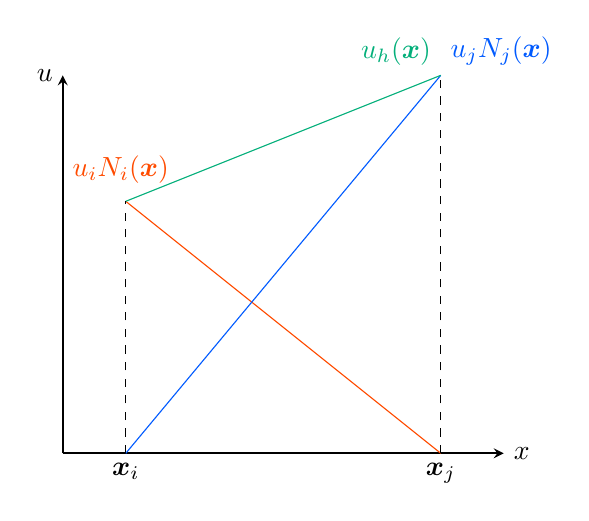
\begin{tikzpicture}[x=4cm,y=4cm]
            \draw[->,>=stealth,semithick] (0,0)--(1.4,0)node[right]{$x$}; %x軸
            \draw[->,>=stealth,semithick] (0,0)--(0,1.2)node[left]{$u$}; %y軸
            %形状関数
            \draw[cud_red](0.2,0.8)--(1.2,0);
            \draw[cud_red] (0,0.9)node[right]{$u_iN_i(\bm{x})$};
            \draw[cud_blue](0.2,0)--(1.2,1.2)node[above right]{$u_jN_j(\bm{x})$};
            \draw[cud_green](0.2,0.8)--(1.2,1.2)node[above left]{$u_h(\bm{x})$};
            %点線とメモリ
            \draw[dashed] (0.2,0)node[below]{$\bm{x}_i$}--(0.2,0.8);
            \draw[dashed] (1.2,0)node[below]{$\bm{x}_{j}$}--(1.2,1.2);
        \end{tikzpicture}
        \caption{形状関数を用いた補間}
        \label{fig:interpolation}
    \end{subfigure}
    \caption{形状関数による補間}
\end{figure}
式\eqref{eq:weak_form}にGalerkin法を適用すると, 
式\eqref{eq:interpolation}の定義より, $u$は定数だから積分の外に出せることに注意して
\begin{align}
    \sum_{j=1}^M\qty[\int_\Omega\nabla N_i\cdot\nabla N_j \dd{\Omega}]u_j
    &= \int_{\partial\Omega_N}N_i f_N\dd{\Gamma} 
    \label{eq:weak_form_galerkin}
\end{align}
を得る. これは$M$本の連立方程式でベクトル表記すると以下の式を得る.
\begin{align}
    \bm{A}\bm{u} &= \bm{f} \\
    A_{ij} &= \int_\Omega\nabla N_i\cdot\nabla N_j \dd{\Omega} \\
    \bm{u} &=
    \begin{Bmatrix}
        u_1\\u_2\\ \vdots \\ u_M
    \end{Bmatrix} \\
    f_{i} &= \int_{\partial\Omega_N}N_i f_N\dd{\Gamma} 
\end{align}
式\eqref{eq:weak_form_galerkin}によると領域全体で積分を行い$\bm{u}$を求められるが,
領域全体で積分するのは実装が難しい.
コードの実装では要素ごとに積分を行ってその後に足し合わせて解を求める.

ここに有限要素法の大きな利点がある.
有限要素法は要素ごとに領域を分割し,
要素内部で立式することができれば,
どのような形状も扱うことができるという強みを持つ.
また, 分割する要素の形状も大きさも一定でなくてよく, 
異なる形状の要素を混在させることもできる.

領域を要素ごとに分割して代数方程式を立てる. 今回は要素はすべて三角形1次要素であるとする.
領域$\Omega$は三角形要素$\Omega^e$で分割される.
したがって弱形式\eqref{eq:weak_form}も要素$\Omega^e$上で成り立つ. 
ここで要素内部での節点番号が全体での節点番号と異なるので, 右上にeをつけて区別する.
\begin{align}
    \int_{\Omega^e} \nabla N^e_i \cdot \nabla N^e_j u^e_j \dd{\Omega}
    &= \int_{\partial\Omega^e_N}N_i f_N\dd{\Gamma} \label{eq:weak_form_elemtnt}
\end{align}
境界条件の導入は全体マトリックスを得た後に行うため, 
Neumann境界条件の積分は境界では場所だと相互に打ち消されるため,
Neumann境界条件はNeumann境界のみになる.

また, Neumann境界条件の導入のしやすさも有限要素法の利点である.
差分法ではNeumann境界条件の導入は煩雑な処理が必要であるが,
有限要素法は差分法よりも簡単に導入できる.
さらに, Neumann境界条件が0の場合(今回だと壁境界, 熱伝導では断熱, 固体力学では外力なし)
は何も処理しなくて導入できるのは大きな利点である.

三角形一次要素は三角形の頂点1, 2, 3, において
\begin{align}
    N^e_i(\bm{x}_j) &= 
    \begin{cases}
        1 & i = j \\
        0 & i \neq j 
    \end{cases}\\
    N^e_1 + N^e_2 + N^e_3 &= 1
\end{align}
を満たす形状関数を持つ.
形状関数$N_i$は
\begin{align}
    N^e_i = a^e_i +b^e_i x +c^e_i y \label{eq:shape_function}
\end{align}
と表される.
係数はそれぞれ
\begin{align}
    \begin{bmatrix}
        1 & x^e_1 & y^e_1 \\
        1 & x^e_2 & y^e_2 \\
        1 & x^e_3 & y^e_3
    \end{bmatrix}
    \begin{bmatrix}
        a^e_1 & a^e_2 & a^e_3 \\
        b^e_1 & b^e_2 & b^e_3 \\
        c^e_1 & c^e_2 & c^e_3
    \end{bmatrix}
    =
    \begin{bmatrix}
        1 & 0 & 0 \\
        0 & 1 & 0 \\
        0 & 0 & 1
    \end{bmatrix}
\end{align}
の関係を満たす. そこで係数について解くと, 
\begin{align}
    a_i = \frac{x_jy_k - x_ky_j}{2|\Omega^e|},\quad
    b_i = \frac{y_j- y_k}{2|\Omega^e|},\quad
    c_i = \frac{x_k - x_j}{2|\Omega^e|} 
    \label{eq:shape_function_coeff}
\end{align}
と表される. ここで$i,j,k$は1,2,3の偶置換\footnote{($(i,j,k)=((1, 2, 3), (2, 3, 1), (3, 1, 2))$)}
であり, $|\Omega^e|$は要素の面積である.

次に式\eqref{eq:weak_form_elemtnt}の弱形式を行列形式にまとめるとこのようになる.
\begin{align}
    \bm{A}^e\bm{u}^e &= \bm{f}^e
\end{align}
ここで$\bm{A}^e$は要素剛性マトリックスと呼ばれ, 以下の式となる.
\begin{align}
    \bm{A}^e_{ij}
    &= \int_{\Omega^e} \qty(\pdv{N_i}{x}\pdv{N_j}{x} + \pdv{N_i}{y}\pdv{N_j}{y}) \dd{V}
    \label{eq:stiffness_matrix_element}
\end{align}
式\eqref{eq:stiffness_matrix_element}は形状関数(式\eqref{eq:shape_function})を代入して
\begin{align}
    \begin{split}
        \bm{A}^e_{ij}
        &= \int_{\Omega^e} \qty(\pdv{N_i}{x}\pdv{N_j}{x} + \pdv{N_i}{y}\pdv{N_j}{y}) \dd{V}  \\
        &= \int_{\Omega^e} (b_ib_j+c_ic_j)\dd{V} \\
        &= (b_ib_j+c_ic_j)|\Omega^e|
        \label{eq:stiffness_matrix_element_solved}
    \end{split}
\end{align}
となる. ここで$|\Omega^e|$は領域の面積である.
$\bm{f}^e$は等価接点流量とよばれる.
\begin{align}
    \bm{f}^e &= \int_{\partial\Omega^e_N}\bm{N}^e f_N\dd{\Gamma}
    \label{eq:nordal_flow}
\end{align}

この積分は計算を解析的に求めることは難しいので, 近似計算で求める.
はじめに要素$e$の境界の積分路を図\ref{fig:element_edges}のように定める.
\begin{figure}[htbp]
    \centering
    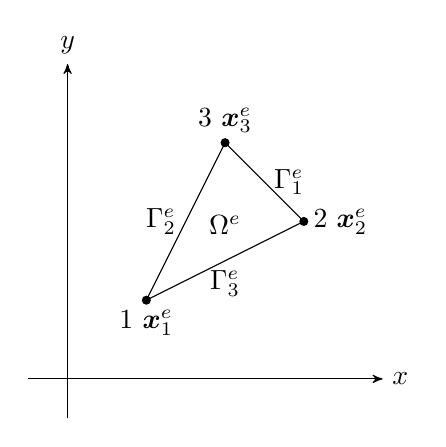
\begin{tikzpicture}[>=stealth']
        \draw[->](-0.5,0) -- (4,0) node[right]{$x$};
        \draw[->](0,-0.5) -- (0,4) node[above]{$y$};
        \filldraw [black] (1,1) circle (0.5mm);
        \filldraw [black] (3,2) circle (0.5mm);
        \filldraw [black] (2,3) circle (0.5mm);
        \draw 
            (1,1)node[below]{1 $\bm{x}^e_1$} --
            (3,2)node[right]{2 $\bm{x}^e_2$} --
            (2,3)node[above]{3 $\bm{x}^e_3$} -- (1,1);
        \draw (2,2.2)node [below]{$\Omega^e$};
        \draw (2,1.5)node[below]{$\Gamma^e_3$};
        \draw (2.5,2.5)node[right]{$\Gamma^e_1$};
        \draw (1.5,2)node[left]{$\Gamma^e_2$};
  \end{tikzpicture}
  \caption{境界の積分路}
  \label{fig:element_edges}
\end{figure}
ここで$\Gamma^e_1$の境界積分を考える.
経路$\Gamma^e_1$は$\bm{x}^e_2$から$\bm{x}^e_3$に向かう経路であり,
その経路はパラメータ$t$を用いて表すと$\bm{\gamma}(t) = \frac{(1+t)}{2}\bm{x}_3 + \frac{(1-t)}{2}\bm{x}_2$となる.
$\Gamma_1$の境界積分は線積分となるので
\begin{align}
    \begin{split}
        \int_{\Gamma^e_1}\bm{N}^e f_N\dd{\Gamma}
        &= \int_{-1}^1 \bm{N}^e(\bm{\gamma}(t))f_N(\bm{\gamma}(t))|\bm{\gamma}(t)|\dd{t} \\
        &= \int_{-1}^1 \bm{N}^e(\bm{\gamma}(t))f_N(\bm{\gamma}(t))\frac{|\bm{x}^e_3-\bm{x}^e_2|}{2}\dd{t}
    \end{split}
\end{align}
を得る.
次にGauss求積という手法を用いて先程の積分を近似する.
Gauss求積は被積分関数$\phi$に対して以下の式で表される.
\begin{align}
    \int_{-1}^1\phi(x)\dd{x}\approx\sum_{i=1}^n w_i\phi(x_i)
\end{align}
有限個の積分点$x_i$に対して重み$w_i$を乗じてその和で近似する.
今回は積分点2点で計算する.
このとき積分点は$\pm\frac{1}{\sqrt{3}}$, 重みは$1$となることが知られている\cite{Yasuda2008}.

他の積分路でも同様の計算が成立するので境界積分が打ち消されない場合,
式\eqref{eq:nordal_flow}は$i,j,k$は$1,2,3$の偶置換として, 以下のように積分を近似できる.
\begin{align}
    \bm{\gamma}_i(t) &= \frac{1+t}{2}\bm{x}^e_k+\frac{1-t}{2}\bm{x}^e_j \\
    \begin{split}
        \bm{f}^e &=\int_{\partial\Omega^e_N}\bm{N}^e f_N\dd{\Gamma} \\
        &= \sum_{i=1}^3 \qty[\int_{-1}^1 \bm{N}^e(\bm{\gamma}_i(t))f_N(\bm{\gamma}_i(t))\frac{|\bm{x}^e_k-\bm{x}^e_j|}{2}\dd{t}] \\
        &\approx\sum_{i=1}^3\qty[\sum_{l=1}^2\bm{N}^e\qty(\bm{\gamma}_i\qty(\frac{(-1)^2}{\sqrt{3}}))f_N\qty(\bm{\gamma}_i\qty(\frac{(-1)^2}{\sqrt{3}}))\frac{|\bm{x}^e_k-\bm{x}^e_j|}{2}]
    \end{split}
\end{align}

さらに先程計算した要素剛性マトリックスから全体剛性マトリックスを求める.
要素剛性マトリックスから全体剛性マトリックスを求める操作はアセンブル操作と呼ばれる.
アセンブル操作の模式図を図\ref{fig:assembling}に示す.
\begin{figure}[htbp]
    \centering
    \includegraphics[width=12cm]{assembling.png}
    \caption{領域ごとのアセンブル操作の概略  Webサイト\cite{Morita2018}より引用}
    \label{fig:assembling}
\end{figure}
具体的なアセンブルのアルゴリズムをアルゴリズム\ref{alg:assembling}に示す.
$\mathrm{nodes}$は接点で$M$個の接点座標の配列で,
$\mathrm{faces}$は要素を指定するノードが並んでいいる2次元配列で,
一つの行に要素の$\mathrm{nodes}$に対するインデックスが3つ並んでいる.
ただし, 上付き文字の文字は配列を意味しない.
\begin{algorithm}
    \caption{Assembling global stiffness matrix}
    \label{alg:assembling}
    \begin{algorithmic}
        \Require $\mathrm{nodes}, \mathrm{faces}$
        \Ensure $A$
        \State $A \leftarrow O$
        \For{$e\leftarrow 1,2,\ldots,N$}
            \For{$i\leftarrow 1,2,3$}
                \State $x^e[i]\leftarrow \mathrm{node}[\mathrm{faces}[e, i]]$    
            \EndFor
            \State calculate $b$, $c$ using eq. \eqref{eq:shape_function_coeff}
            \For{$i,j\leftarrow 1,2,3$}
                \State $A^e[i,j] \leftarrow (b[i]b[j]+c[i]c[j])|\Omega^e|$
            \EndFor 
            \For{$i,j\leftarrow 1,2,3$}
                \State $A[\mathrm{faces}[e,i],\mathrm{faces}[e,j]] \leftarrow A[\mathrm{faces}[e,i],\mathrm{faces}[e,j]] + A^e[i,j]$
            \EndFor
        \EndFor
    \end{algorithmic}
\end{algorithm}
また, $A$は疎行列となるので, 多くの場合は$A$をCSR (Compressed Sparse Row)形式や
CSC (Compressed Sparse Column)形式で格納される.

なお, 局所等価接点流量ベクトルも同様に全体等価接点流量ベクトルをアセンブル操作ができる.

最後にDirichlet条件の代入を行う.
接点$i$がDirichlet条件$u_D$だった場合を述べる.
連立方程式を解いたときもその条件が維持される必要があるので
$i$行目は$u_i=u_D$が成立して, 他の行に$u_i$の項が含まれないようにする.
また, 全体剛性行列は対象行列であるという性質が数値計算の上では便利であるため,
対称性を残す.
これら2つの要件をアルゴリズムにするとアルゴリズム\ref{alg:zero_clear}が得られる.
\begin{algorithm}
    \caption{Applying Dirichlet boundary condition}
    \label{alg:zero_clear}
    \begin{algorithmic}
        \Require $A \in\mathbb{R}^{M\times M}$, $f \in\mathbb{R}^{M}$, $i$, $u_D$
        \Ensure $A$, $f$
        \State $A[i,i] \leftarrow 1$
        \State $f[i] \leftarrow u_D$
        \For{$j\neq i$}
            \State $A[i, j] \leftarrow 0$ 
            \State $f[j] \leftarrow  f[j] - A[j,i]u_D $
            \State $A[j,i] \leftarrow 0$
        \EndFor
    \end{algorithmic}
\end{algorithm}
疎行列のデータ形式は0の領域を保存せずに圧縮するので0の入った項を最後に削除するコードを実装するとよい.

\section{翼型の生成}
今回は計算対象として翼型のまわりの流れを計算する. 
翼型はさまざまなものがあるが, 
NACA翼型の一つであるNACA 2412を用いる.
NACA翼型はNACA(National Advisory Committee for Aeronautics, 
連邦航空諮問委員会, NASAの前身)が開発した翼型である.

文献\cite{Rinoie2011}を参考にNACA 2412を説明する.
NACA 2412はNACA 4桁翼型と呼ばれるグループに属しており, 翼型断面が多項式で定義されている.
翼型の厚み分布$y_t$, 前縁半径$r_t$, 翼型中心線$y_c$を用いて定義する.
\begin{align}
    y_t &= 5t \qty(0.2969 \sqrt{x} - 0.1260 x - 0.3516 x^2 + 0.2843 x^3 - 0.1015 x^4) \\
    r_t &= 1.1019t^2 \\
    y_c &=
    \begin{cases}
        \frac{m}{p^2}(2px-x^2),& 0\leq x\leq p\\
        \frac{2m}{(1-p)^2}[(1-2p)+2px-x^2],& p< x\leq 1
    \end{cases}
\end{align}
また, パラメータとして
\begin{itemize}
    \item $x$ : 翼弦の相対的な位置(前縁を0とし, 後縁を1とする)
    \item $m$ : 翼型の厚みの比(翼型の番号の1000の位を100で割る, 今回は$m=0.02$)
    \item $p$ : 反りが最大になる$x$の値(翼型の番号の100の位を10で割る, 今回は$p=0.4$)
    \item $t$ : 翼型の最大厚みの比(翼型の番号の下二桁を100で割る, 今回は$t=0.12$)
\end{itemize}
がある.
主翼の上半分を構成する曲線を$(x_U,y_U)$とし, 下半分を構成する曲線を$(x_L,y_L)$とする.
このとき,
\begin{align}
    x_U &= x-y_t\sin{\theta},&y_U &= y_c+y_t\cos{\theta}\\
    x_L &= x+y_t\sin{\theta},&y_L &= y_c-y_t\cos{\theta}
\end{align}
と定義される\cite{Abbott1945}.
ここで$\theta$は翼型中心線の接線と$x$軸のなす角で,
\begin{align}
    \theta &= \arctan{\dv{y_c}{x}} \\
    \dv{y_c}(x) &= 
    \begin{cases}
        \frac{2m}{p^2}(p-x), & 0\leq x\leq p \\
        \frac{2m}{(1-p)^2}(p-x) & p <x\leq 1
    \end{cases}
\end{align}

\section{結果と考察}
計算結果が解析解と定性的に一致しており, 正しく問題を解くことができたと考えられる.

\clearpage
\printbibliography[title=参考文献]

\appendix
\section{諸々の計算}
\subsection{速度ポテンシャルの存在}
\label{appendix:potential}
以下の式で定義される関数$\Phi$が速度ポテンシャルであることを示す.
\begin{align}
    \Phi(\bm{x}) &= \int_O^{\bm{x}} \bm{u}\cdot\mathrm{d}\bm{l} \label{eq:potential:def}
\end{align}
非圧縮かつ定常でその上渦なし完全流体が流れている場を考察する.
場の内部に2点$P,Q$があり, $P$から出発して$Q$で終わる異なる曲線$C_1$, $C_2$があり,
$C_1$と$C_2$で囲まれる領域が曲面となっているものとする.
点$P$から$C_1$を通って点$Q$にいたり, 点$Q$から$C_2$を通って点$P$に戻る積分路を考える.
この周回積分の値は式\eqref{eq:stokes:zero}より0となることが示されるので
\begin{align}
    \oint_{C_1-C_2}\bm{u}\cdot\mathrm{d}\bm{l} &= 0 \\
    \int_{C_1}\bm{u}\cdot\mathrm{d}\bm{l}-\int_{C_2}\bm{u}\cdot\mathrm{d}\bm{l} &=0\\
    \int_{C_1}\bm{u}\cdot\mathrm{d}\bm{l}&=\int_{C_2}\bm{u}\cdot\mathrm{d}\bm{l}
\end{align}
以上の式変形から, 式\eqref{eq:potential:def}で定めた関数$\Phi$の値は積分路に依存しない.
よって関数$\Phi$がポテンシャルである.

\subsection{Gauss-Greenの定理}
\label{appendix:gauss_green}
Gaussの発散定理
\begin{align}
    \int_\Omega\nabla\cdot\bm{A}\dd{\Omega} =\int_{\partial\Omega}\bm{A}\cdot\bm{n}\dd{\Gamma}
    \label{eq:divergence_theorem}
\end{align}
に対して$\bm{A}=\phi\nabla\psi$を代入し, 式変形をしてGauss-Greenの定理を得る.
\begin{align}
    \int_\Omega\nabla\cdot(\phi\nabla\psi)\dd{\Omega} 
    &=\int_{\partial\Omega}\phi\nabla\psi\cdot\bm{n}\dd{\Gamma} \\
    \int_\Omega(\phi\nabla^2\psi+\nabla\phi\cdot\nabla\psi)\dd{\Omega} 
    &=\int_{\partial\Omega}\phi\nabla\psi\cdot\bm{n}\dd{\Gamma} \\
    \int_\Omega\phi\nabla^2\psi\dd{\Omega} 
    &=- \int_\Omega\nabla\phi\cdot\nabla\psi\dd{\Omega}
    +\int_{\partial\Omega}\phi\nabla\psi\cdot\bm{n}\dd{\Gamma}
\end{align}

\section{ボツになった内容}
\subsection{Zhukovsky変換を用いた翼の生成}
Zhukovsky変換を用いて翼型を生成した. 
現在の旅客機ではスーパークリティカル翼型をベースに設計されているが
\cite{Rinoie2011}\footnote{2次元翼型については文献\cite{Rinoie2011}の5章が詳しい},
簡単な変数変換によって生成でき, 
2次元翼理論による結果の検証がしやすいためこれを用いる.

Zhukovsky変換は複素平面$\zeta$から複素平面$z$に対して
以下の複素関数で変換を行うものである.
\begin{align}
    z = \zeta +\frac{1}{\zeta}
\end{align}
この変換の特徴として, $z$を円とすると$z$が翼型になるということと,
$\zeta\neq 0$において正則関数になる特徴がある.
今回は$\zeta$を以下のように定めた.
\begin{align}
    |\zeta- \zeta_0| = |c-\zeta_0|
\end{align}
ここで, $\zeta_0 = -0.1+0.1i$, $c=1$と定めた.

Julia言語でZhukovsky変換を実装したコードをリストに示し, 
画像を図\ref{fig:zhukovsky}に示す.
\begin{figure}[htbp]
    \centering
    \includegraphics[width=8cm]{zhukovsky_aerofoil.pdf}
    \caption{Zhukovsky変換の結果}
    \label{fig:zhukovsky}
\end{figure}

\end{document}